
%%%%%%%%%%%%%%%%
% Autoencoders %
%%%%%%%%%%%%%%%%

\section{Autoencoders}
\label{sec:auto}



% PCA vs autoencoder %
%%%%%%%%%%%%%%%%%%%%%%

\subsection{PCA vs autoencoder}

\textbf{Principal Component Analysis} (or PCA) is a statistical technique that is used to transform a set of (potentially) correlated data vectors into a (smaller) number of linearly uncorrelated variables---the Principal Components (PCs). They are sorted in such a way that the first PC accounts for the largest amount of variability, and each subsequent PC covers a maximal portion of the remaining variance while remaining orthogonal with the preceding PCs.

The principal component decomposition of a data matrix $\mathbf{X}$ (with $n$ rows and $p$ columns) is described by

\begin{equation} \label{eq:1}
	\mathbf{T} = \mathbf{XW}
\end{equation}

where $\mathbf{W}$ is a $p \times p$ matrix of weights whose columns are the eigenvectors of $\mathbf{X^ \intercal X}$. 

Not all PCs need to be retained for PCA to be a useful tool. More specifically, PCA is often used as a means of dimensionality reduction, by projecting the data vectors onto a subset of all PCs---more specifically, the K first PCs. Equation \ref{eq:1} becomes:

\begin{equation} \label{eq:2}
	\mathbf{T_L} = \mathbf{XW_L}
\end{equation}

The goal of PCA can then be described as finding a projection so that the best linear reconstruction of the data is as close as possible to the original data. Keeping in mind that the inverse of an orthogonal matrix equals its transpose, this translates to

\begin{equation} \label{eq:3}
	\mathbf{L_{PCA}} = \norm{\mathbf{X} - \mathbf{T_L W ^\intercal_L  }}_2^2
\end{equation}

This statistical method is closely related to a specific type of neural network---the \textbf{linear autoencoder (LA)} (see figure \ref{fig:linear_autoencoder}). This neural network takes a data vector as input, passes it through a single hidden layer (typically smaller in dimensionality than the input), and attempts to reconstruct the data in the output layer using linear activation functions. As such, the network is forced to learn an optimal strategy in order to minimize the reconstruction loss.

\begin{figure}[htbp]
	\begin{center}
		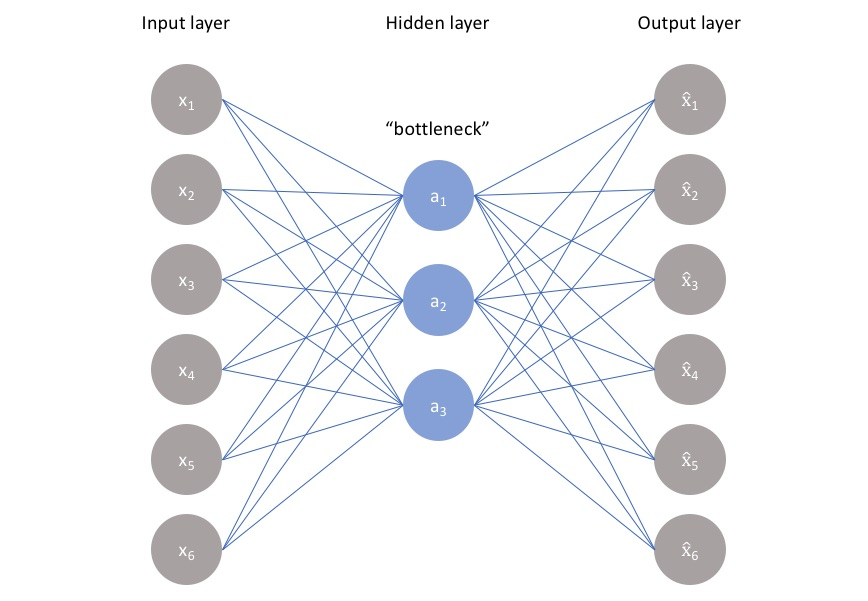
\includegraphics[width=\linewidth]{images/autoencoder.jpg}
		\caption{Linear autoencoder architecture with input dimension 6, encoding dimension 3, and compression factor 2 (taken from \textcolor{blue}{\url{https://www.jeremyjordan.me/autoencoders/}}).}
		\label{fig:linear_autoencoder}
	\end{center}
\end{figure}

From intuition, we can assume that this optimal strategy involves two things: 1) each node in the encoded (hidden) layer must cover a maximal amount of variability, and 2) the contribution of the nodes to the output must overlap as little as possible. It is already apparent that this mission is heavily related to the workings of PCA. 

Suppose we built a linear autoencoder for the same data matrix $\mathbf{X}$. This data is passed on to the hidden layer, when then passes the transferred data on to the output layer. Defining two successive activation functions $f$ and $g$, this process can be described by the following equations.

\begin{equation} \label{eq:4}
	\mathbf{Z} = f(\mathbf{W_1 X})
\end{equation}
\begin{equation}\label{eq:5}
	\mathbf{\hat{X}} = g(\mathbf{W_2 Z})
\end{equation}

By definition, training this network means attempting to minimize the reconstruction loss.  Given the linearity of the activation functions $f$ and $g$, this is described by:

\begin{equation} \label{eq:6}
	\mathbf{L_{LA}} = \norm{\mathbf{X} - \mathbf{W_2 W_1 X}}_2^2 
\end{equation}

We can see that optimizing the weight matrix for this linear autoencoder for all intents and purposes equates to the solution for PCA (\ref{eq:3}).

A difference between both approaches can be found in the boundaries of the dimensionality. In linear autoencoders, the hidden layer can be made up of more nodes than the input and output layers, meaning that the data is transformed to a feature space greater than the original input space. PCA, on the other hand, can never yield more PCs than the dimensionality of the input space.



% Nonlinear and convolutional %
%%%%%%%%%%%%%%%%%%%%%%%%%%%%%%%

\subsection{Nonlinear and convolutional}
\label{sec:auto2}

In this section, two distinct autoencoders are described\footnote{The code for this section can be found in \texttt{scripts/itnodl\_auto.py}.}. The first autoencoder has a linear architecture---it thus consists of an input layer, output layer, and a single hidden layer. A second autoencoder is created by training a deep convolutional neural network. The architecture for both autoencoders is shown in figures \ref{fig:auto1} and \ref{fig:auto2}. 

\begin{figure}[!htbp]
	\begin{center}
		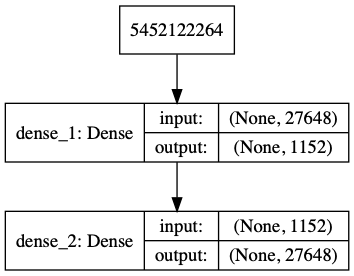
\includegraphics[width=8cm, height=6cm, keepaspectratio]{images/auto_lin_architecture}
		\caption{Linear architecture for autoencoder 1. Input and output dimensions $96\times96\times3 = 27648$, compression factor 24, encoding dimension 1152.}
		\label{fig:auto1}
	\end{center}
\end{figure}

\begin{figure}[!htbp]
	\begin{center}
		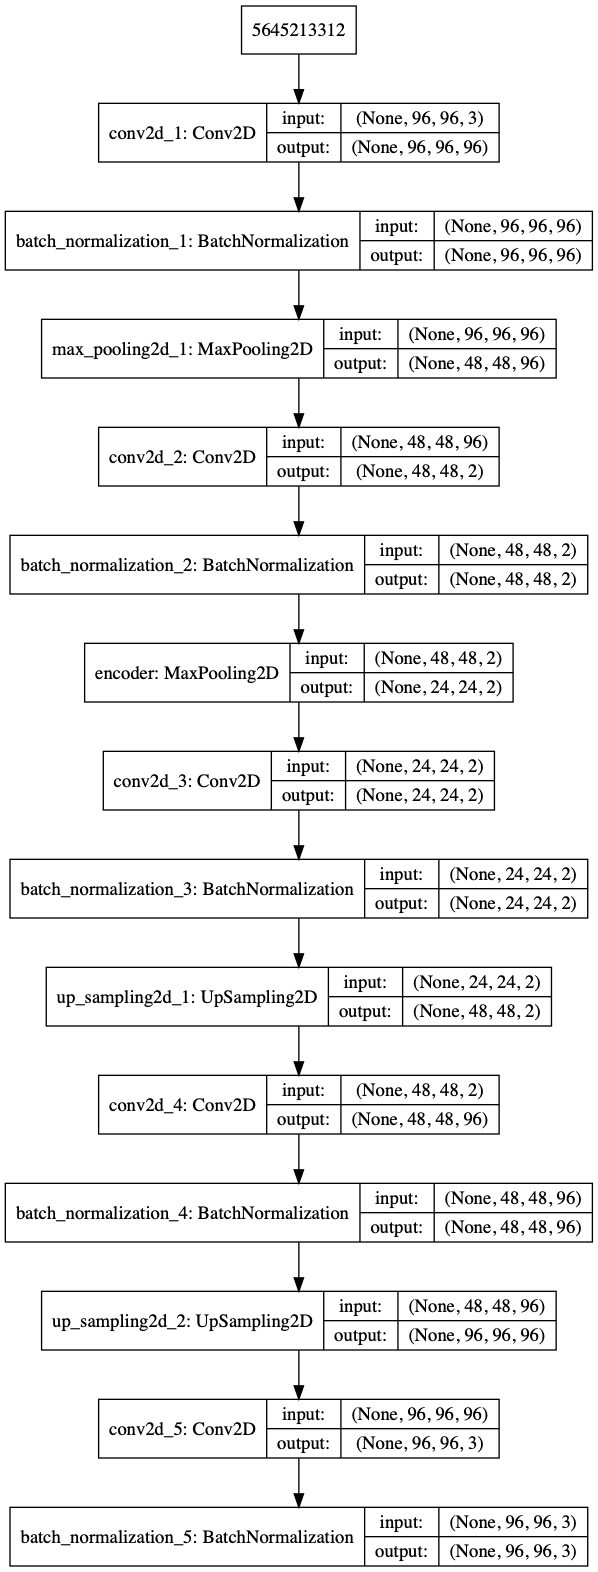
\includegraphics[height=20cm, keepaspectratio]{images/auto_conv_architecture}
		\caption{Deep convolutional architecture for autoencoder 2. Same input, output, and encoding dimensions as autoencoder 1.}
		\label{fig:auto2}
	\end{center}
\end{figure}

\paragraph{Architectures} The \textit{linear autoencoder} consisted of an input layer, output layer, and a hidden layer. Its transfer functions were, of course, both linear. The \textit{deep convolutional autoencoder}, in turn, was made up of 5 convolutional layers, each of them using a $3 \times 3$-sized kernel. The kernel values were initialized in a random uniform manner, and bias was initialized to zero. After each convolutional layer, batch normalization was applied to accelerate and stabilize the training process. The data was downsampled after each convolutional layer preceding the encoded layer (using max pooling), and then upsampled back to attain the original image dimensions. All transfers were modeled by \textit{ReLU} (Rectified Linear Unit), except for the final activation---there, a sigmoid transfer function was used. The main advantages of using \textit{ReLU} in the intermediate layers are:

\begin{itemize}

	\item{\textit{ReLU} is a mathematically simple, and thus computationally cheap transfer function. This implies less strain on the CPU during training (a sorely needed benefit).}
	\item{\textit{ReLU} will likely converge faster during training, since the function slope doesn't 'plateau', as can be the case when using \textit{sigmoid} or \textit{tanh} transfer functions.}
	\item{Since \textit{ReLU} is defined as zero for negative input values, it is a sparsely activated transfer function---it is likely that not all input causes activation, which translates to a lower computational demand.}

\end{itemize}

The final layer uses a sigmoid activation function, since we require output in the $[0, 1]$ range.

\paragraph{Network parameters} A number of parameters were equal in both autoencoder networks. The models were each designed to accept $96\times96\times3$-sized images as input, and were trained to reconstruct the images in those same dimensions. The 'bottleneck' layer in the middle of the networks---capturing the encoded representation---consisted of 1152 nodes, corresponding with a compression factor of 24. The encoding dimension was chosen after some experimentation: I ran the model with different values, and observed the evolution of the loss function as well as the eventual reconstructed images. Both models were set to train for \textit{200 epochs}. If no improvement was detected in the validation loss for 20 epochs, training \textit{stopped early}. This was implemented to avoid overfitting. In training, I used an \textit{Adam} optimizer algorithm (default parameters), and chose \textit{mean squared error} to compute reconstruction loss. 

\begin{figure}[!htbp]
	\begin{center}
		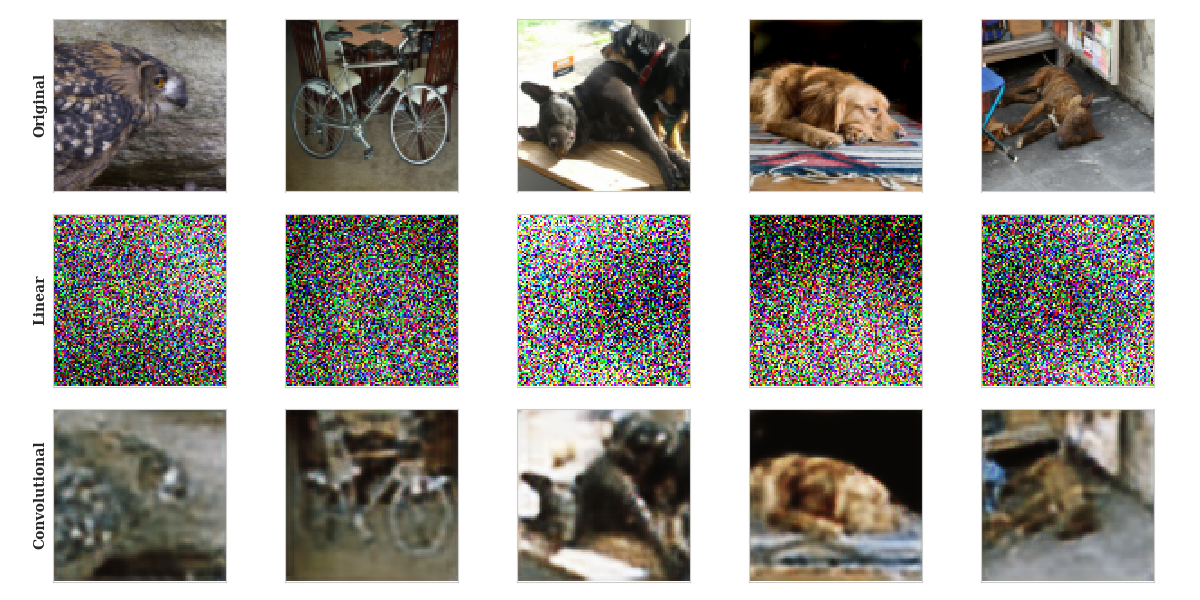
\includegraphics[width=\linewidth, keepaspectratio]{images/auto_reconstruction}
		\caption{Image reconstructions yielded by both autoencoders for a random selection of 5 'fresh' test images ($96\times96\times3$ pixels). The top row shows the original images. The middle and bottom row show the reconstructions made by the linear autoencoder and deep convolutional autoencoder, respectively.}
		\label{fig:auto_visual}
	\end{center}
\end{figure}

\begin{figure}[!htbp]
	\begin{center}
		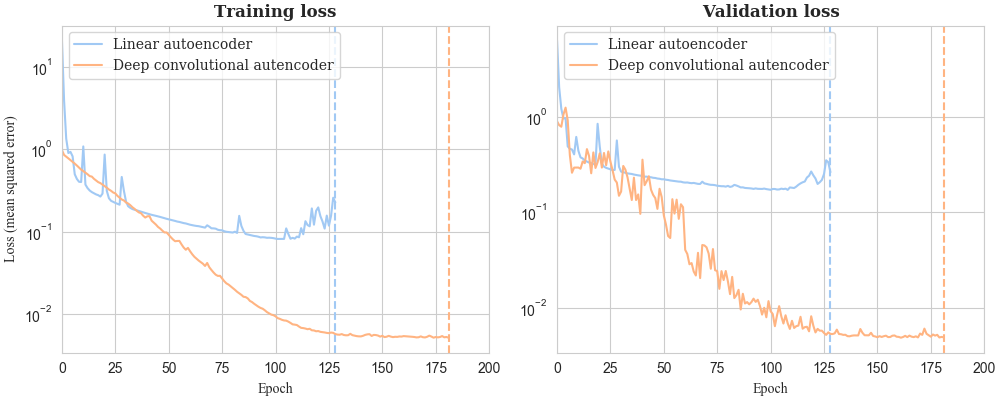
\includegraphics[width=\linewidth, keepaspectratio]{images/auto_histories}
		\caption{Training history for both autoencoders. The left graph shows the evolution of the loss (mean squared error) on the training data, whereas the right graph shows the evolution of the validation loss. The vertical dotted line indicates when early stopping occurred, due to a lack of improvement in the latter value. Loss is expressed on a logarithmic scale.}
		\label{fig:auto_histories}
	\end{center}
\end{figure}

\paragraph{Evaluation} Both autoencoders only differed in terms of model architecture---all training parameters, and the size of the encoded layer, were equal. The results, however, are quite different. Visual inspection of each model's predictions shows that the deep convolutional neural network (DCNN) is distinctly better at preserving the characterizing features of the original image (see figure \ref{fig:auto_visual}), or reconstructing anything that resembles the input image for that matter. Figure \ref{fig:auto_histories} displays the training history of both models. Several observations can be made: 

% Please add the following required packages to your document preamble:
% \usepackage{booktabs}
\begin{table}[!htbp]

	\renewcommand{\arraystretch}{1.5}
	\centering
	
\begin{tabular}{@{}cccc@{}}

	
\toprule
                        Model      & \textbf{Train}  & \textbf{Validation} & \textbf{Test}   \\ \midrule
\textbf{\textit{Linear autoencoder}}            & \num{1.77e-1}   & \num{2.62e-1}       & \num{2.73e-1}   \\
\textbf{\textit{Deep convolutional autencoder}} & \num{5.12e-3} & \num{4.92e-3}     & \num{5.14e-3} \\ \bottomrule

\end{tabular}
\caption{Evaluation of models based on reconstruction loss: \textit{mean squared error} values for training, validation and test datasets.}
\label{tab:auto_eval}
\end{table}


\begin{itemize}
	\item The deep convolutional autoencoder took a longer time to converge to an optimal solution (under the early stopping criteria) compared to the linear autoencoder. This is unsurprising, given the different number of training parameters---there are a lot more options for the DCA to improve and fine-tune its reconstruction strategy.
	\item The final DCA model was characterized by a significant lesser amount of loss, compared to the LA model (see table \ref{tab:auto_eval}). This quality difference is also apparent from the visual reconstruction of the test images (figure \ref{fig:auto_visual}).
	\item The evaluation table (table \ref{tab:auto_eval}) shows that, for the LA, the reconstruction loss is higher for the evaluation and test images, compared to the training image reconstruction loss. The DCA, on the other hand, shows a fairly constant loss over all datasets, seen and unseen. This implies that the DCA was better at capturing the underlying, example-agnostic features, whereas the LA's learnt strategy was more limited to the images it was presented with during training.
\end{itemize}

\paragraph{Latent space visualization} There are several options to visualize the space of the encoded representations. One option is to take the decoding part of the network---that is, the encoded layer serves as input layer, and constructs an image based on the latent representation it receives. Presenting this decoder subnetwork with a 'one-hot encoded' input vector would then generate an 'eigenface'. This is feasible when the latent space is limited in dimensionality, otherwise we need a way to rank the importance of the encoded features (if that is at all possible). In case of LA, this translates to finding the eigenvalues of the weight matrix. In case of DCA, such an approach is not so straightforward.
